% Options for packages loaded elsewhere
\PassOptionsToPackage{unicode}{hyperref}
\PassOptionsToPackage{hyphens}{url}
%
\documentclass[
]{article}
\usepackage{amsmath,amssymb}
\usepackage{lmodern}
\usepackage{ifxetex,ifluatex}
\ifnum 0\ifxetex 1\fi\ifluatex 1\fi=0 % if pdftex
  \usepackage[T1]{fontenc}
  \usepackage[utf8]{inputenc}
  \usepackage{textcomp} % provide euro and other symbols
\else % if luatex or xetex
  \usepackage{unicode-math}
  \defaultfontfeatures{Scale=MatchLowercase}
  \defaultfontfeatures[\rmfamily]{Ligatures=TeX,Scale=1}
\fi
% Use upquote if available, for straight quotes in verbatim environments
\IfFileExists{upquote.sty}{\usepackage{upquote}}{}
\IfFileExists{microtype.sty}{% use microtype if available
  \usepackage[]{microtype}
  \UseMicrotypeSet[protrusion]{basicmath} % disable protrusion for tt fonts
}{}
\makeatletter
\@ifundefined{KOMAClassName}{% if non-KOMA class
  \IfFileExists{parskip.sty}{%
    \usepackage{parskip}
  }{% else
    \setlength{\parindent}{0pt}
    \setlength{\parskip}{6pt plus 2pt minus 1pt}}
}{% if KOMA class
  \KOMAoptions{parskip=half}}
\makeatother
\usepackage{xcolor}
\IfFileExists{xurl.sty}{\usepackage{xurl}}{} % add URL line breaks if available
\IfFileExists{bookmark.sty}{\usepackage{bookmark}}{\usepackage{hyperref}}
\hypersetup{
  pdftitle={Declining-population paradigm},
  pdfauthor={NRES 470/670},
  hidelinks,
  pdfcreator={LaTeX via pandoc}}
\urlstyle{same} % disable monospaced font for URLs
\usepackage[margin=1in]{geometry}
\usepackage{graphicx}
\makeatletter
\def\maxwidth{\ifdim\Gin@nat@width>\linewidth\linewidth\else\Gin@nat@width\fi}
\def\maxheight{\ifdim\Gin@nat@height>\textheight\textheight\else\Gin@nat@height\fi}
\makeatother
% Scale images if necessary, so that they will not overflow the page
% margins by default, and it is still possible to overwrite the defaults
% using explicit options in \includegraphics[width, height, ...]{}
\setkeys{Gin}{width=\maxwidth,height=\maxheight,keepaspectratio}
% Set default figure placement to htbp
\makeatletter
\def\fps@figure{htbp}
\makeatother
\setlength{\emergencystretch}{3em} % prevent overfull lines
\providecommand{\tightlist}{%
  \setlength{\itemsep}{0pt}\setlength{\parskip}{0pt}}
\setcounter{secnumdepth}{-\maxdimen} % remove section numbering
\ifluatex
  \usepackage{selnolig}  % disable illegal ligatures
\fi

\title{Declining-population paradigm}
\author{NRES 470/670}
\date{Spring 2021}

\begin{document}
\maketitle

{
\setcounter{tocdepth}{2}
\tableofcontents
}
\textbf{Q}: Is the intrinsic rate of growth \(r_{max}\) positive or
negative for most species on earth? Why???

\textbf{Q}: Given that most species are capable of sustained growth and
attaining large population size under favorable conditions, how do
populations get small in the first place? Why are many populations
declining despite their intrinsic ability to grow? Is it all random, or
is it more systematic?

\hypertarget{threats-to-populations}{%
\subsection{Threats to populations}\label{threats-to-populations}}

The answer of course is that the intrinsic ability to grow under ideal
conditions is not the whole story. Populations are stocks with inflows
and outflows- and if mortalities exceed births \emph{under present
conditions} the population will decline until these unfavorable
conditions are reversed.

In the ``small-population paradigm'' lecture, we discussed several
\textbf{stochastic threats} to populations, including loss of genetic
diversity (genetic drift), demographic stochasticity, catastrophic
environmental events. These threats only really affect small
populations. Large populations are mostly resilient to stochastic
threats.

Large populations can be threatened too though! Factors that threaten
large populations are generally called \textbf{deterministic threats}!

The \textbf{declining population paradigm} focuses on the factors that
make large populations small -- that is, it is the \emph{study of those
deterministic processes that cause population decline (that tip the
balance and cause deaths to exceed births), and how these processes may
be reversed through effective conservation management}.

What are some factors that can \emph{tip the balance} so to speak- so
that growing or stable populations become declining populations?

\hypertarget{over-harvest}{%
\subsubsection{Over-harvest}\label{over-harvest}}

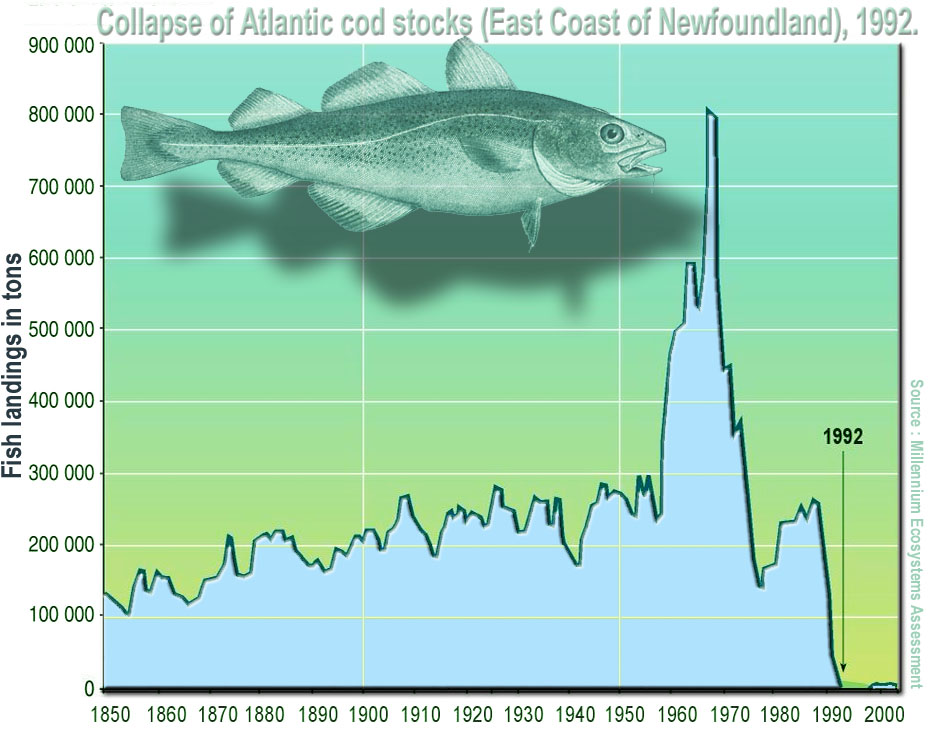
\includegraphics{overharvest1.jpg}

\hypertarget{habitat-loss-and-degradation}{%
\subsubsection{Habitat loss and
degradation}\label{habitat-loss-and-degradation}}

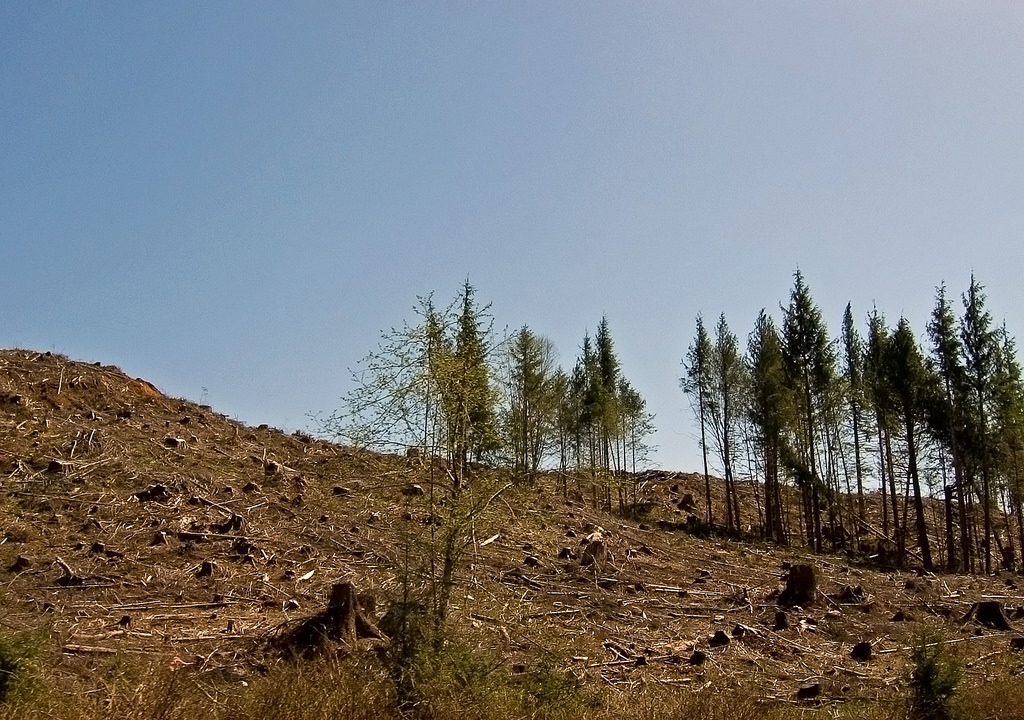
\includegraphics{habitatloss1.jpg}

\hypertarget{pathogens-and-parasites}{%
\subsubsection{Pathogens and parasites}\label{pathogens-and-parasites}}

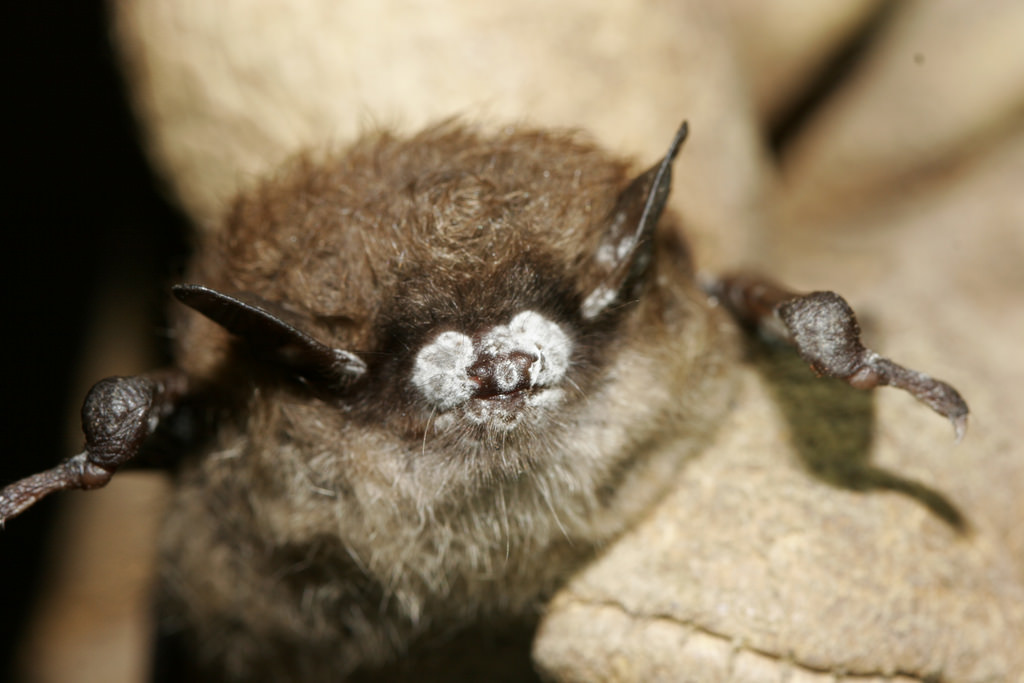
\includegraphics{whitenose1.jpg}

\hypertarget{climate-change}{%
\subsubsection{Climate change}\label{climate-change}}

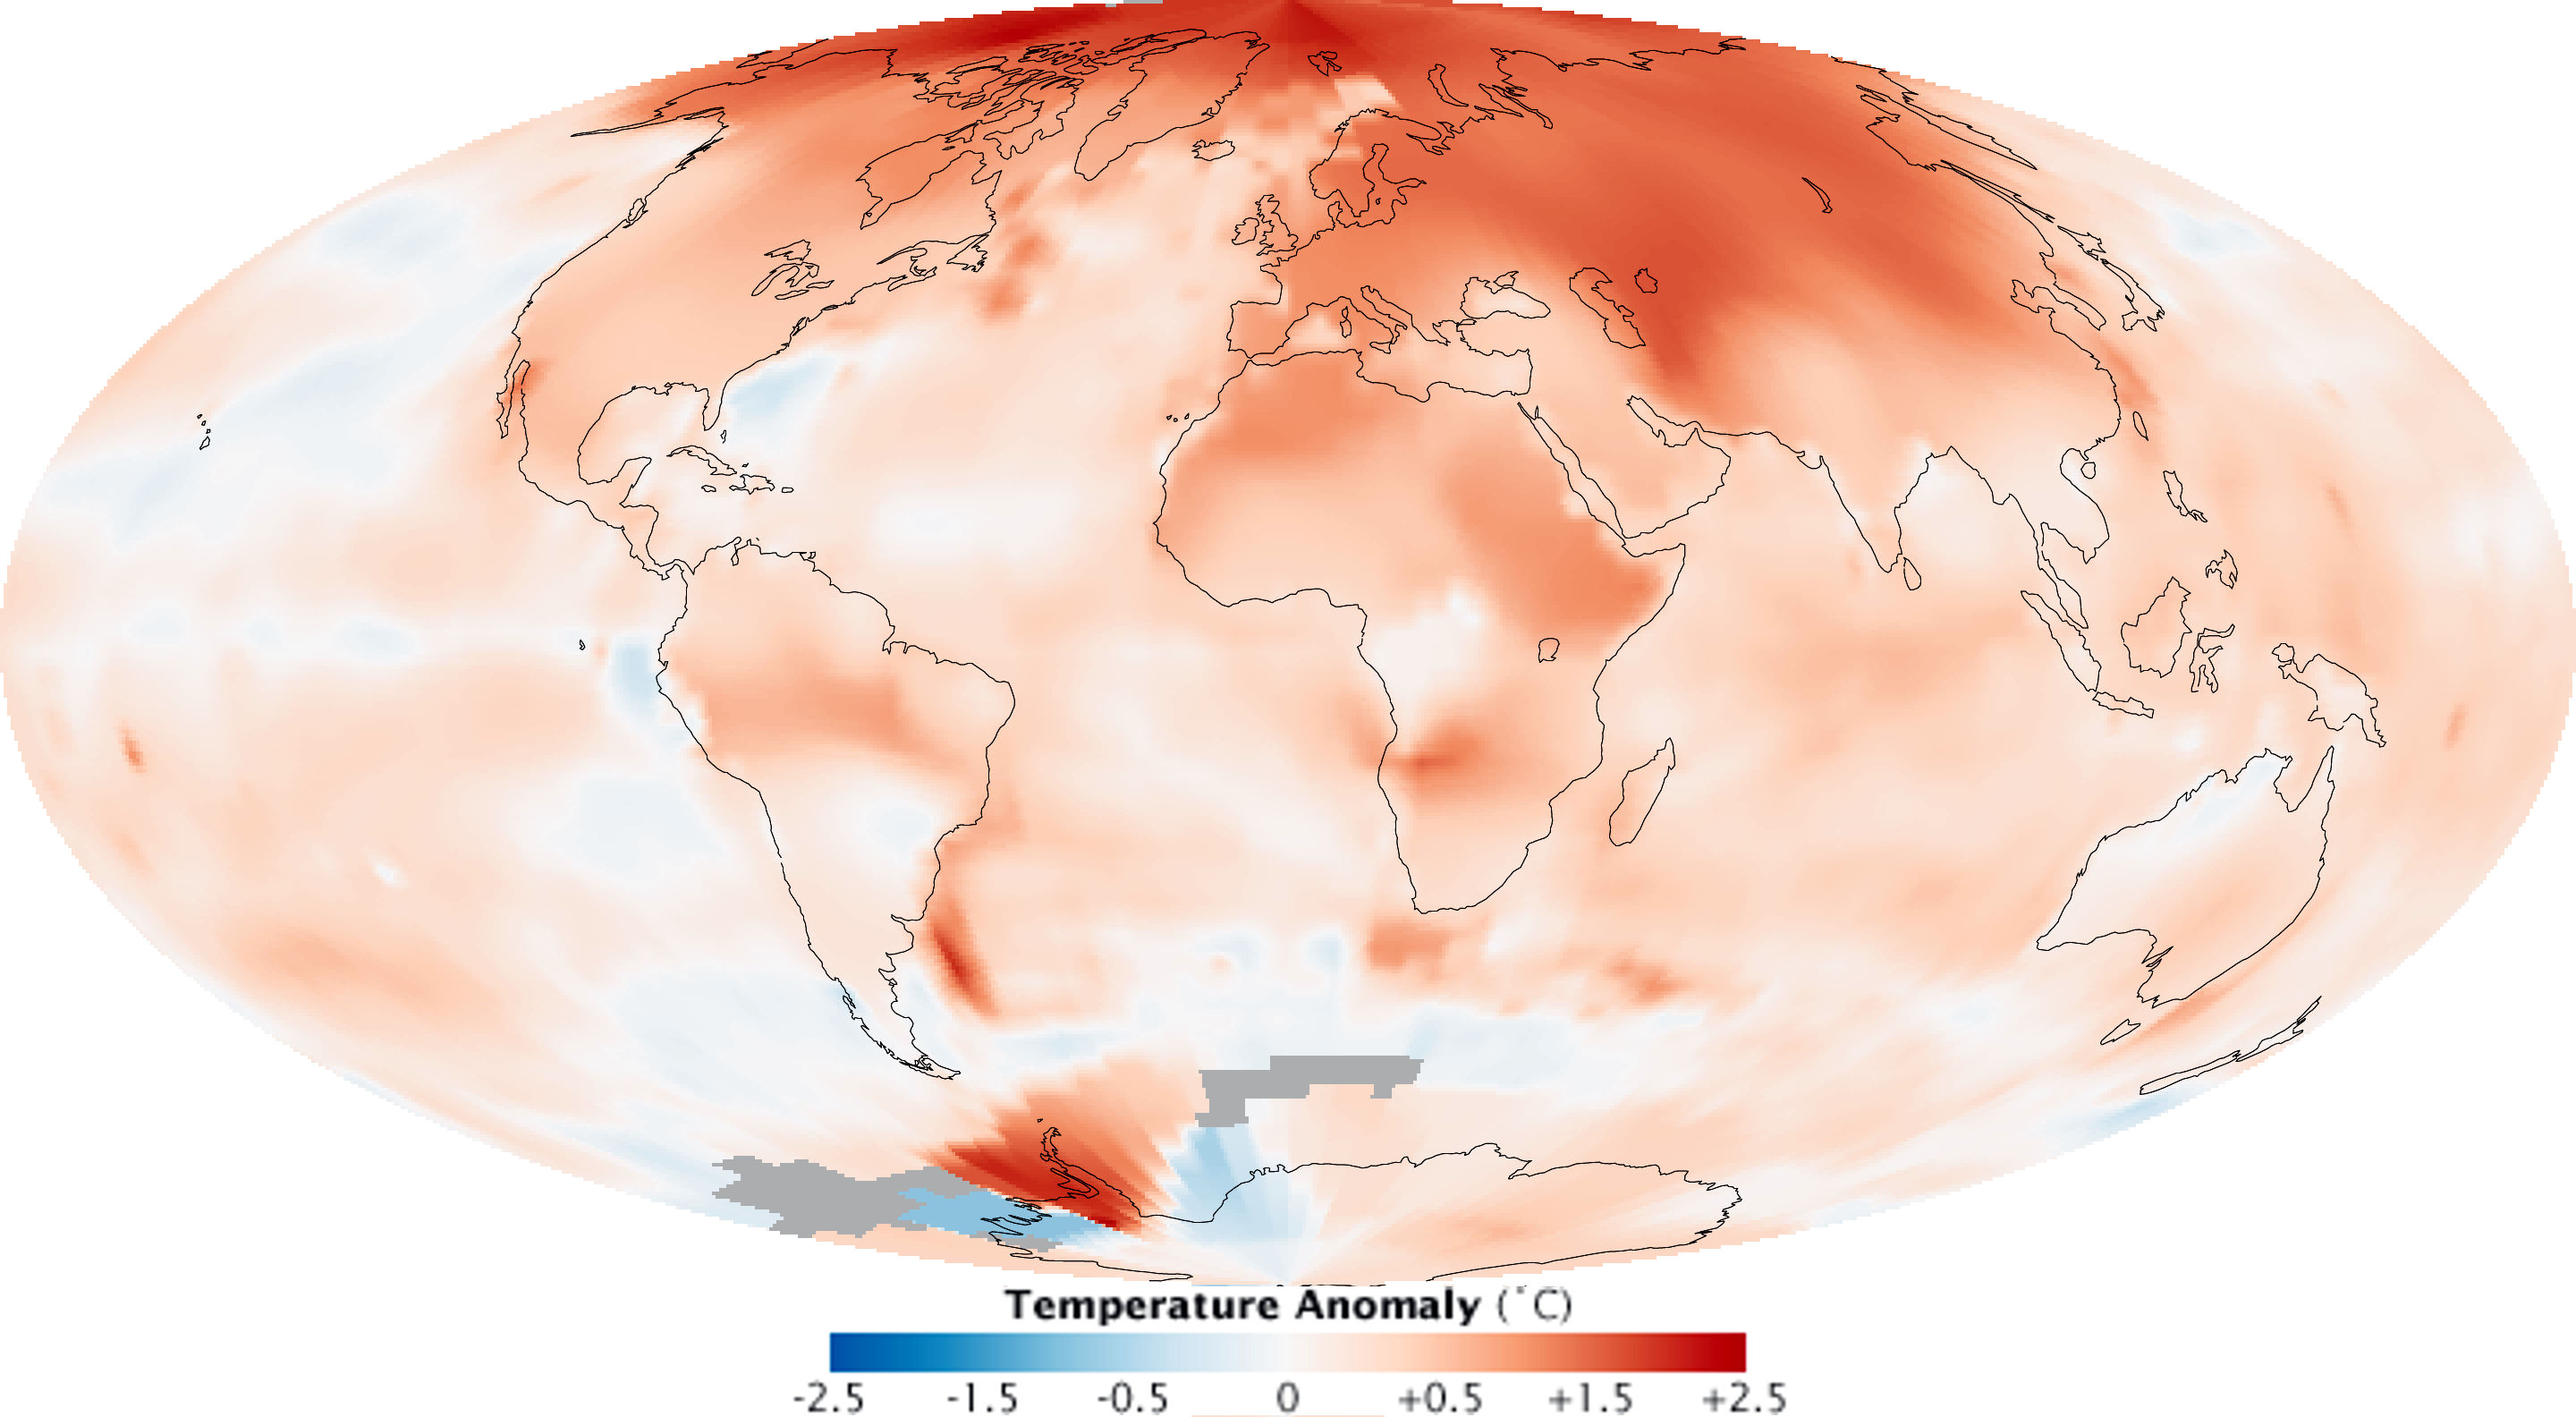
\includegraphics{climatechange1.jpg}

This map shows the difference (anomaly) between current temperatures and
mean (normal) temperatures recorded since 1880.

\hypertarget{exotic-invasive-species}{%
\subsubsection{Exotic invasive species}\label{exotic-invasive-species}}

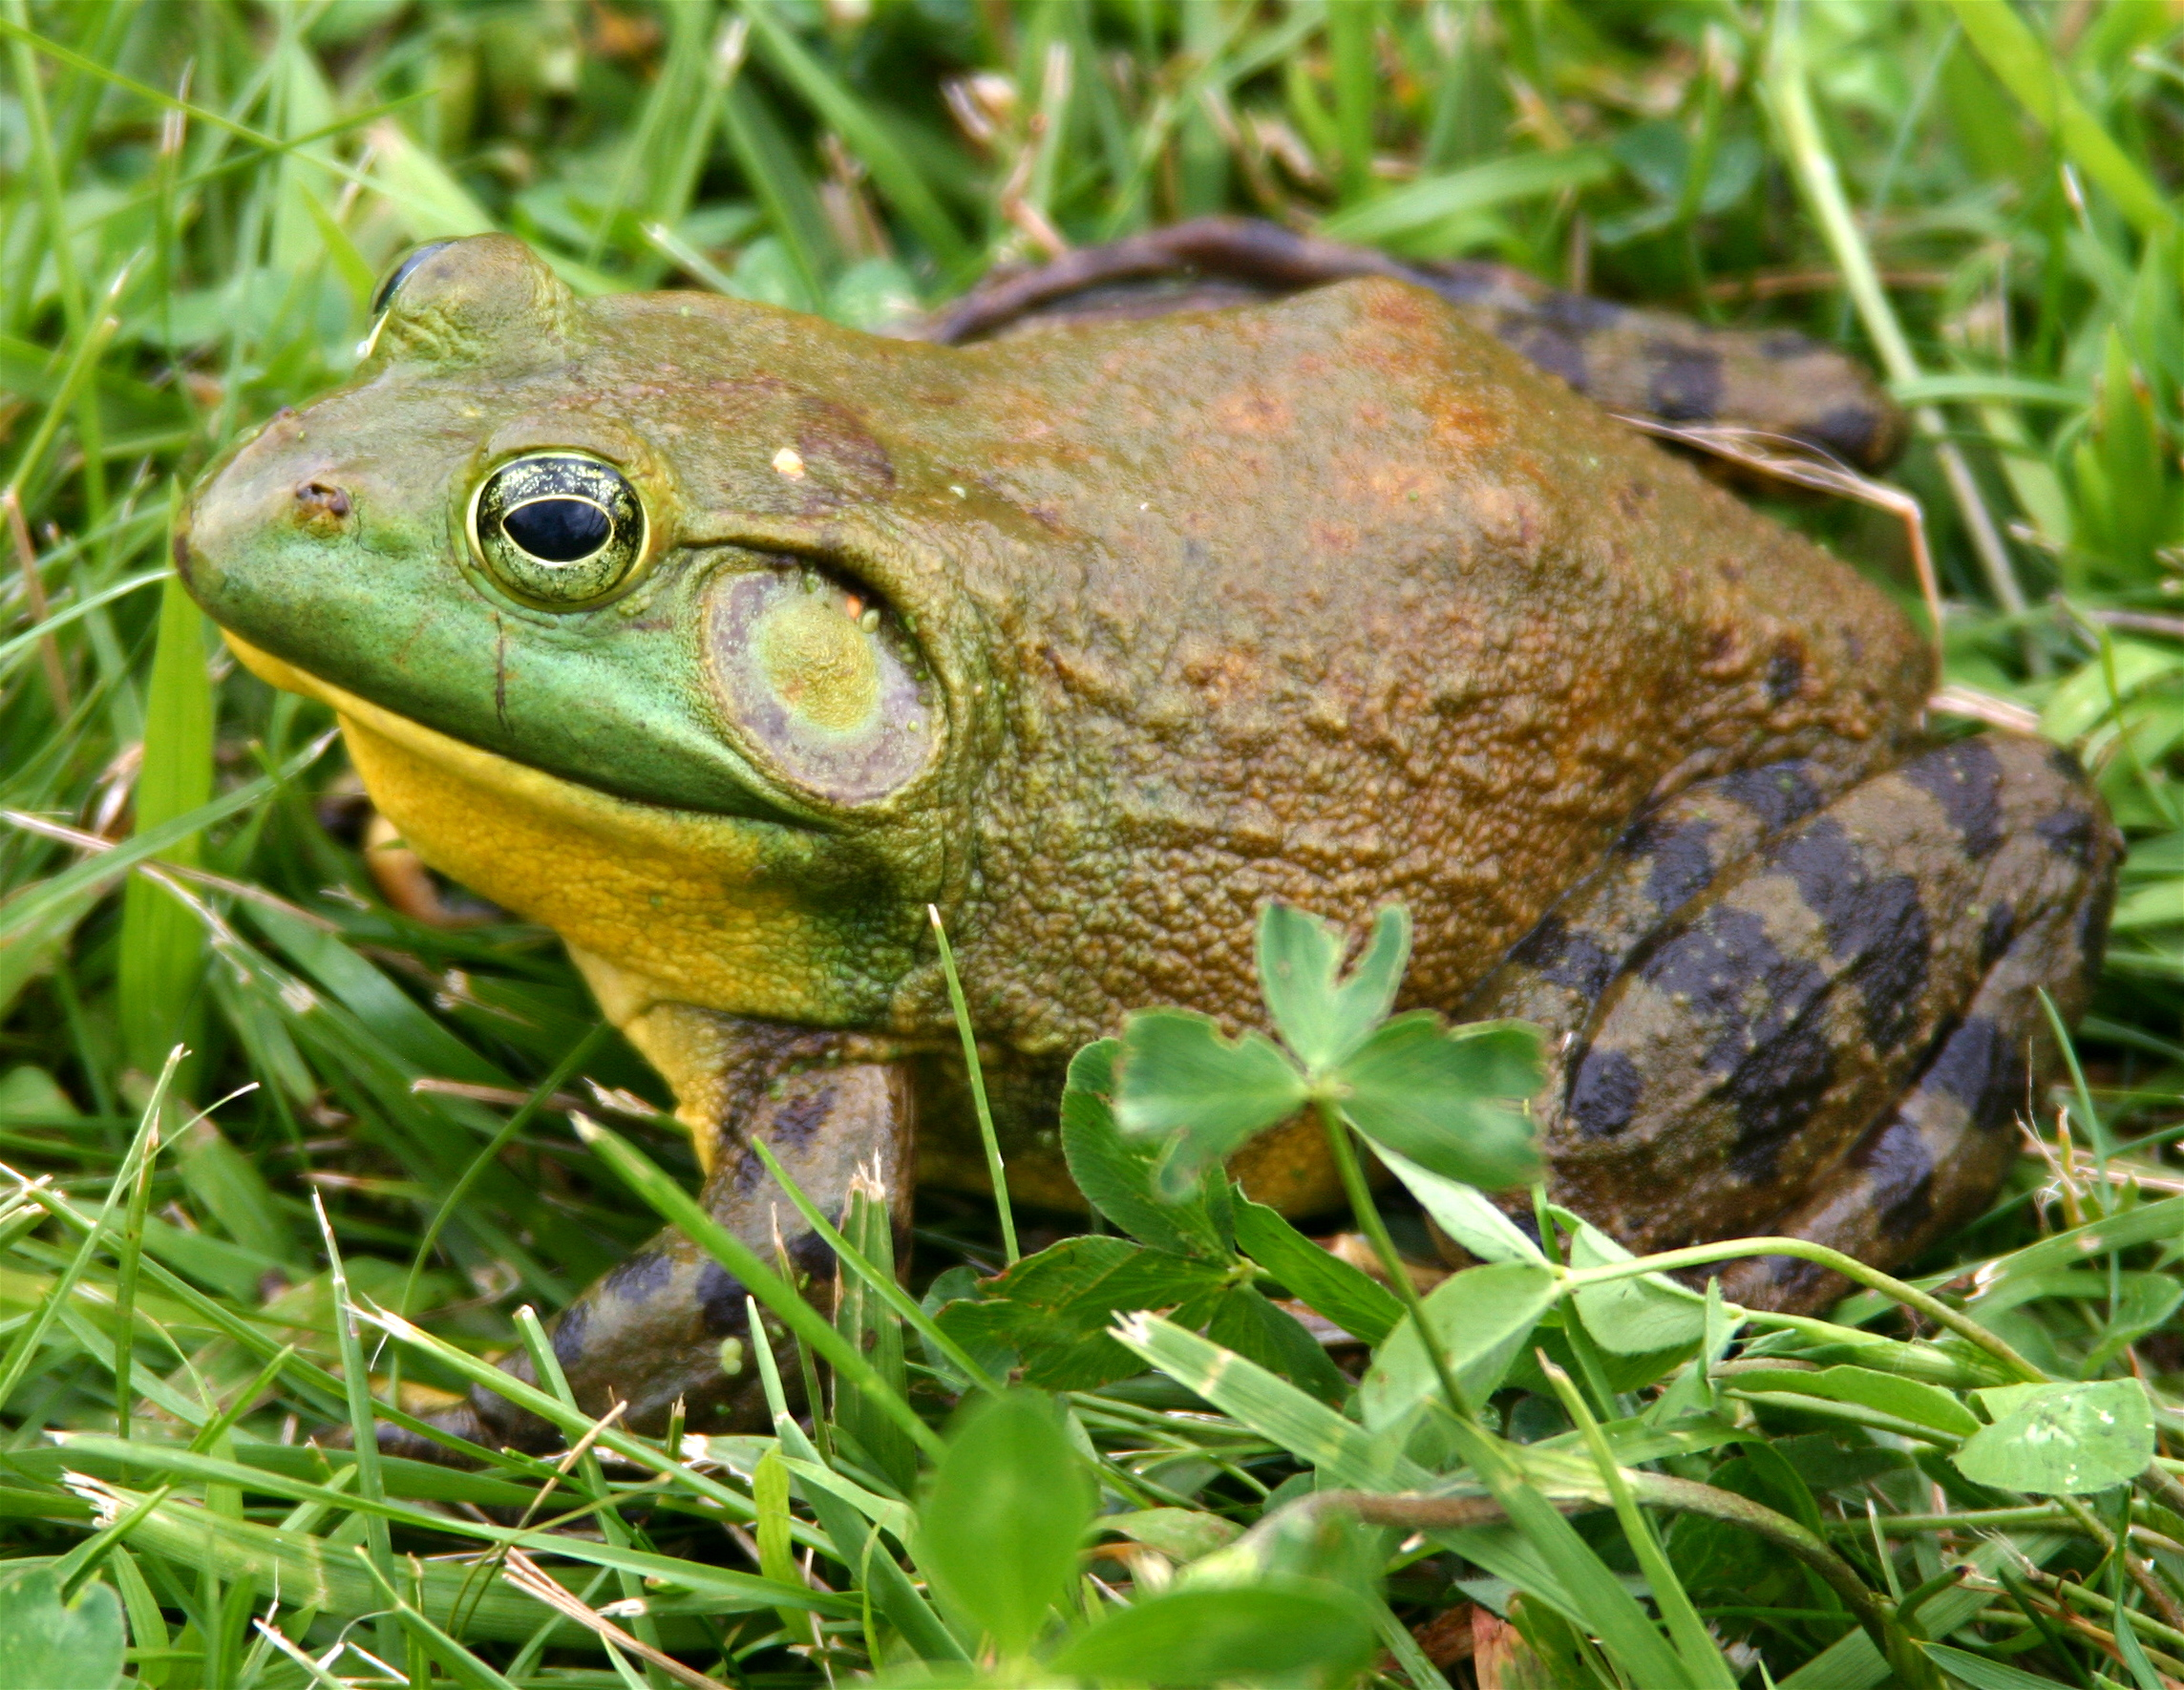
\includegraphics{bullfrog1.jpg}

\hypertarget{pollution}{%
\subsubsection{Pollution}\label{pollution}}

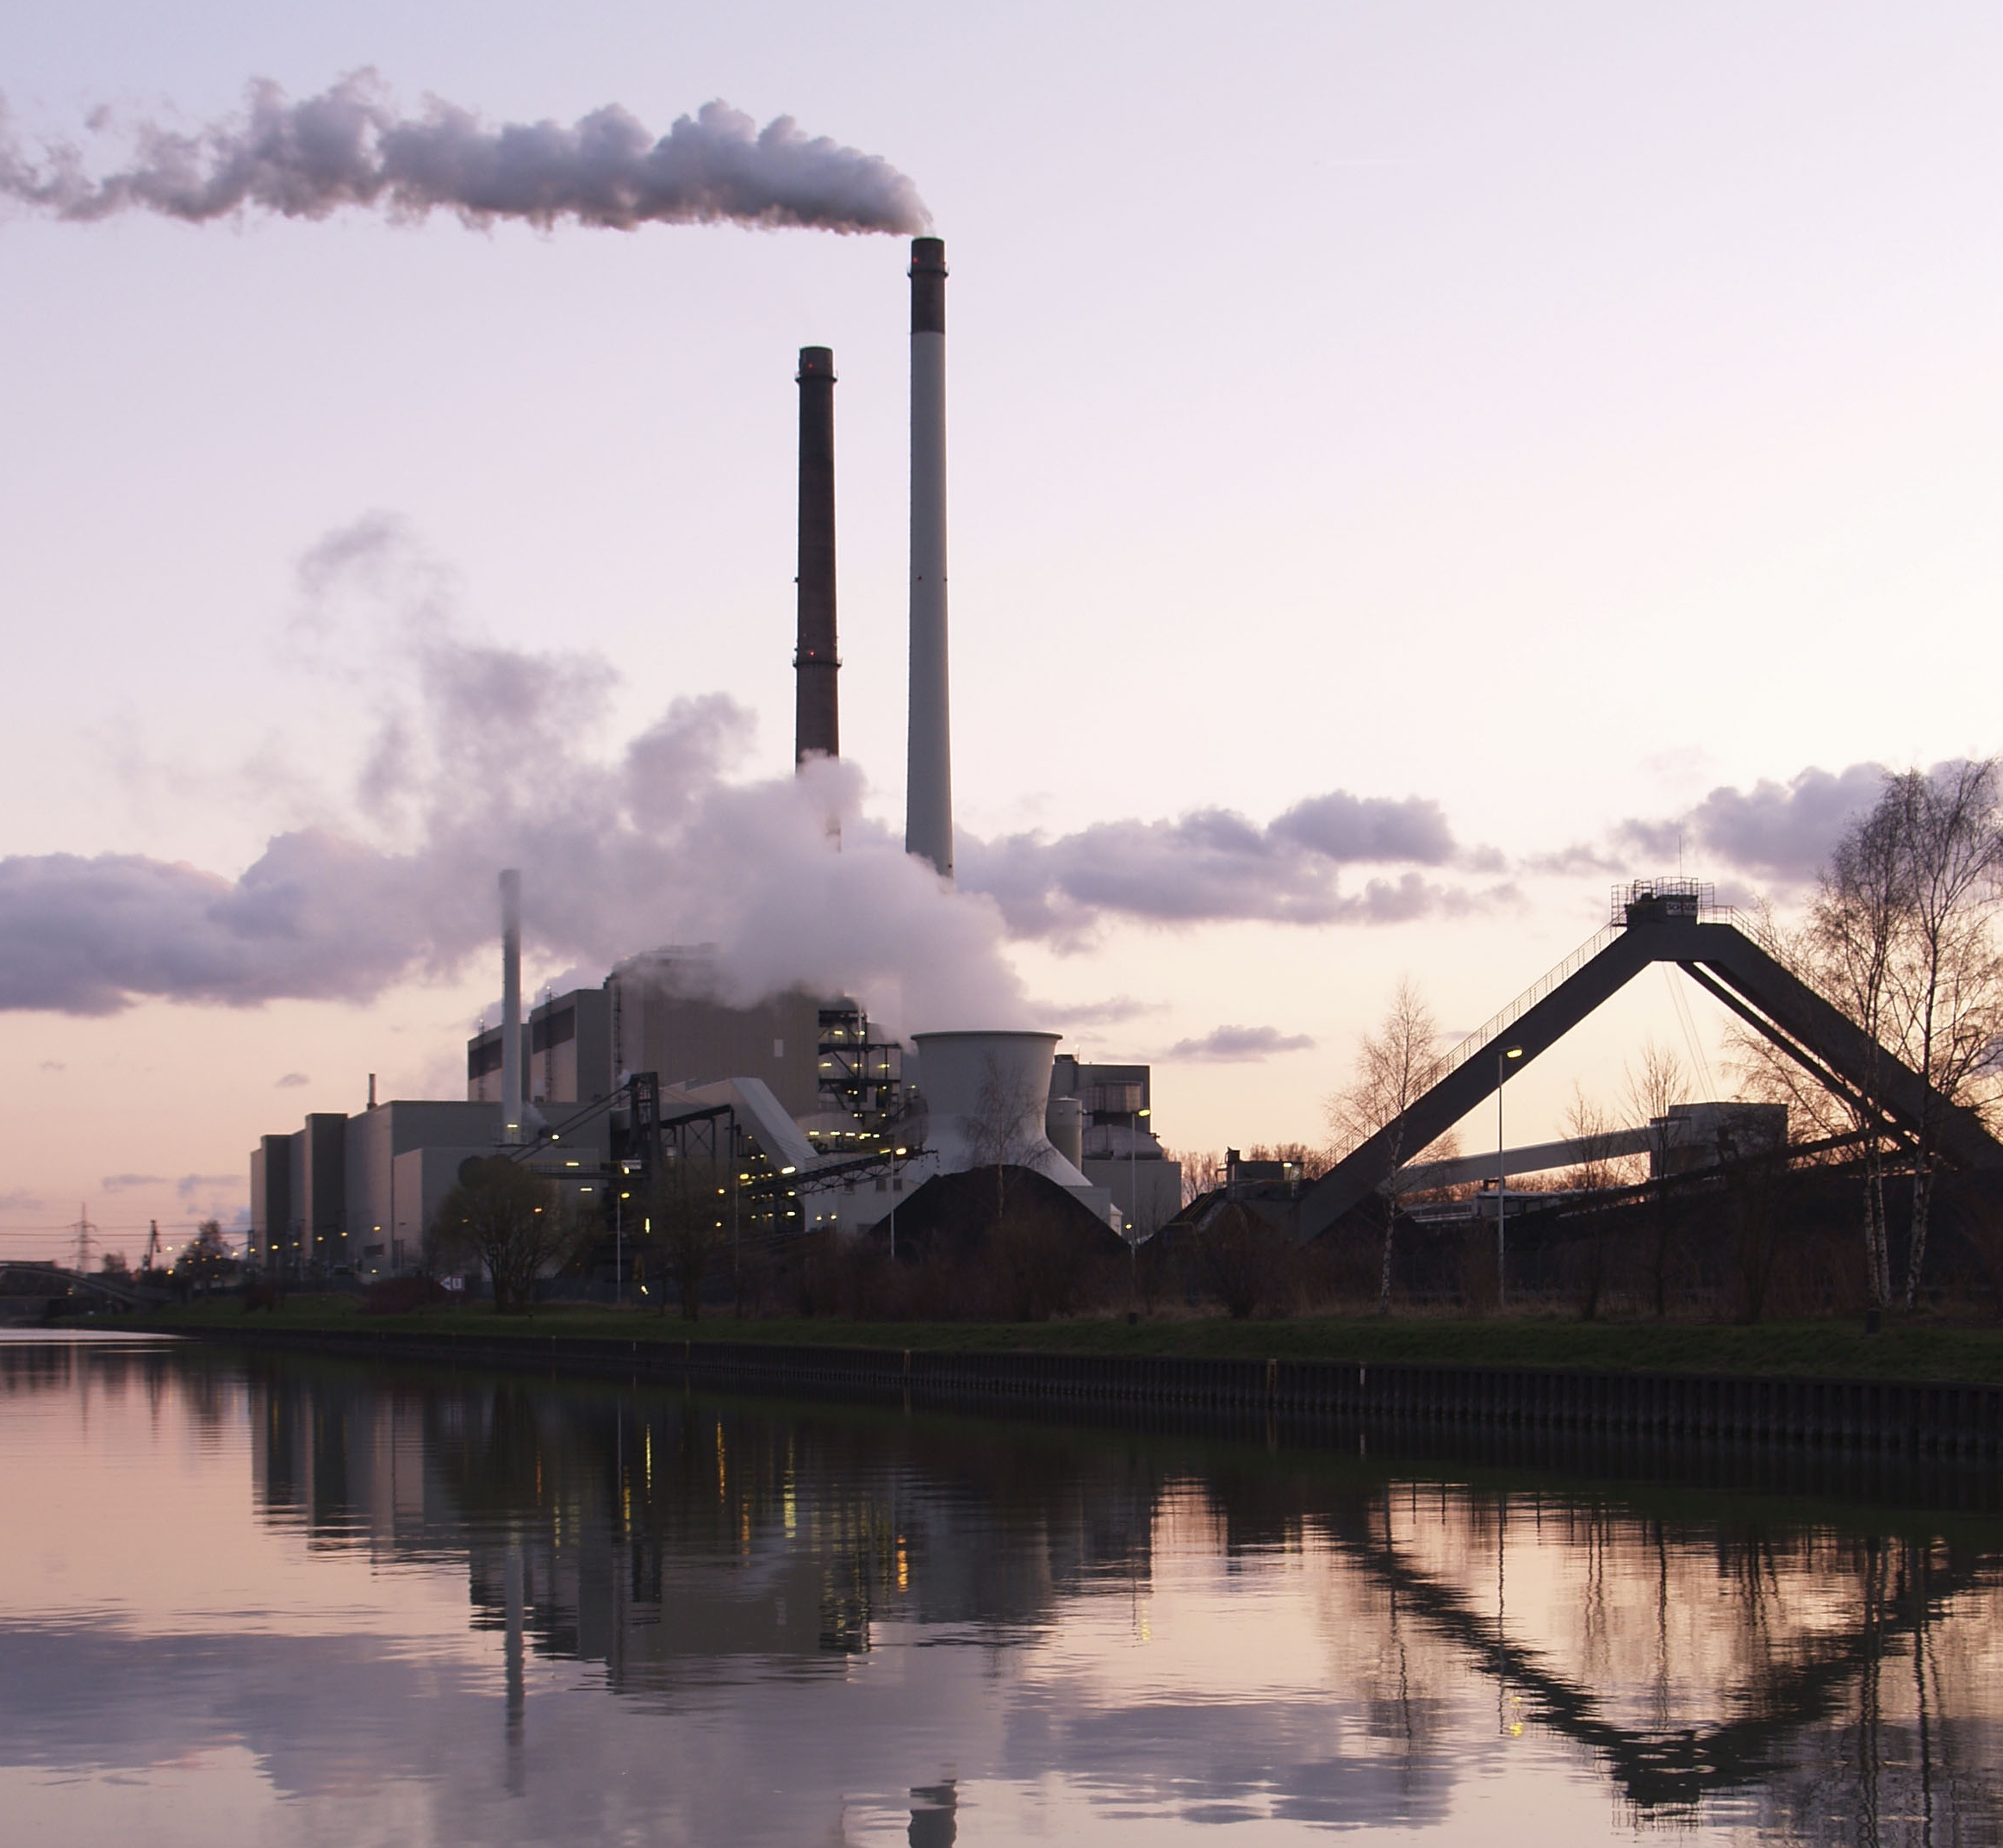
\includegraphics{pollution1.png}

\hypertarget{the-debate-in-conservation-biology}{%
\subsection{The debate in Conservation
Biology!}\label{the-debate-in-conservation-biology}}

So, which one is more important for conservation? The
declining-population paradigm or the small-population paradigm??

This ``controversy'' was ignited by a \href{caughley1.pdf}{very
influential paper by Graeme Caughley} in \emph{Journal of Animal
Ecology} in 1994.

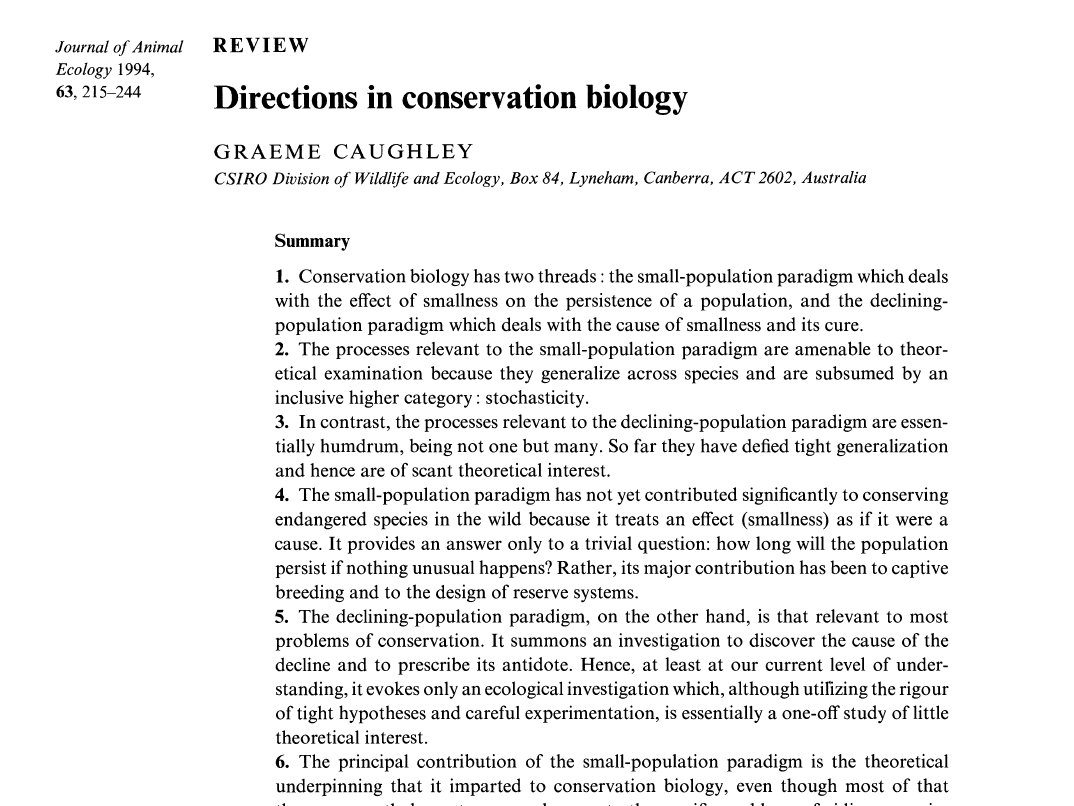
\includegraphics{caughley1.jpg}

In this paper, Caughley coined the terms `small population paradigm' and
`declining population paradigm', and expressed a strong bias towards one
paradigm and against the other\ldots{}

\begin{quote}
Conservation biology has two threads: the small-population paradigm
which deals with the effect of smallness on the persistence of a
population, and the declining- population paradigm which deals with the
cause of smallness and its cure.
\end{quote}

\textbf{Q}: Can you detect Caughley's bias in the above quote?

\textbf{Q}: What do you think? Do you agree with Caughley? Take a moment
to look over the paper and please comment on TopHat!

\hypertarget{in-class-exercise-deterministic-threats}{%
\subsubsection{In-Class Exercise: Deterministic
threats}\label{in-class-exercise-deterministic-threats}}

Let's try a worked example to illustrate the above points.

Let's start with a souped up scalar, density-dependent population --
should look something like this:

You can clone this model by clicking
\href{https://insightmaker.com/insight/74417/declining-population-paradigm}{here}

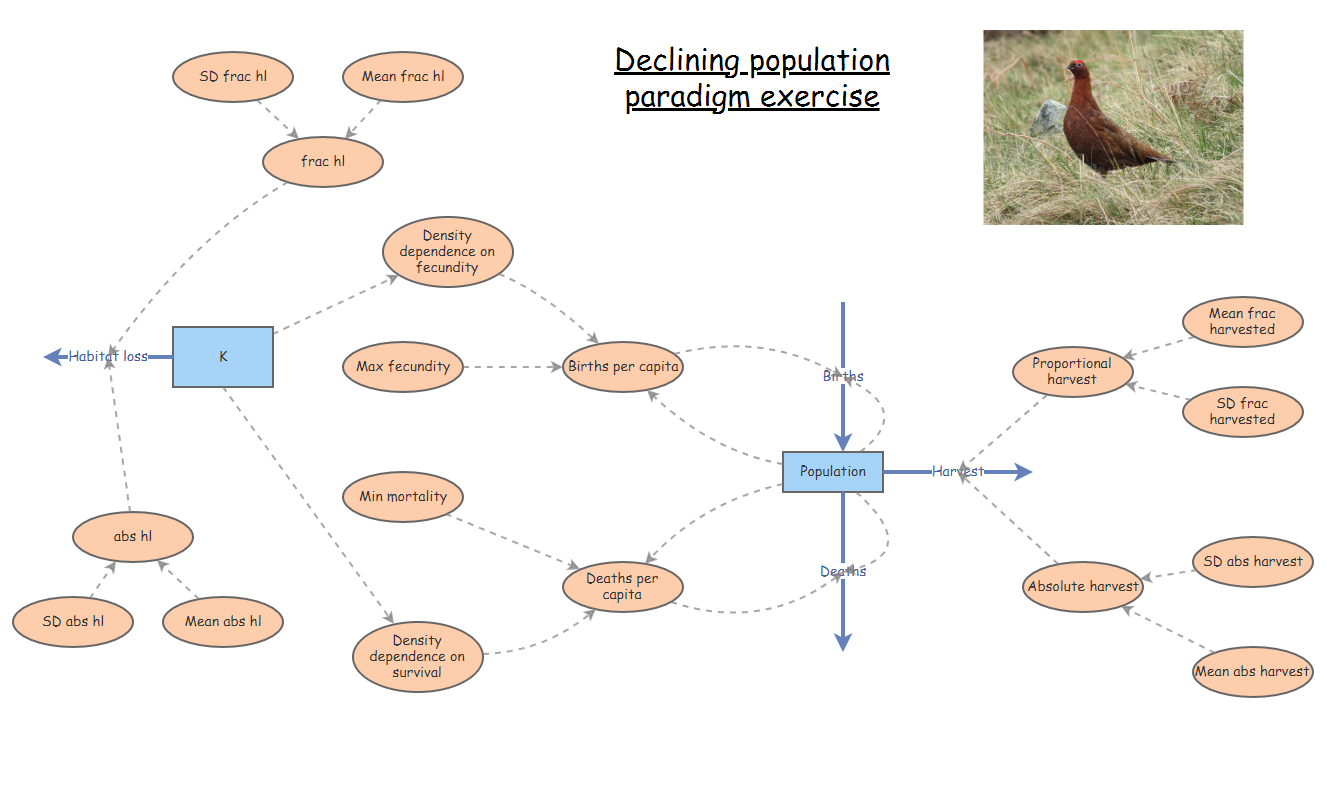
\includegraphics{IM5.PNG}

You should see logistic growth (with demographic stochasticity) if you
hit the simulate button. Take a minute to run the base model and make
sure you understand how it works.

For this exercise, let's change the initial population to 200 (half of
K).

Also, make sure that the time step is 1 year, and the model should run
for 50 years.

\textbf{Let's add a harvest process!}

\begin{itemize}
\tightlist
\item
  Assume that approximately 10\% of the population is harvested each
  year (a fractional harvest). However, the true harvest rate is
  stochastic and \emph{normally distributed}- occasionally harvest goes
  as high as 15\%, and occasionally as low as 5\%. Make sure you specify
  the `fractional harvest' parameters (mean and stdev) in the model so
  that you achieve this range.
\end{itemize}

\textbf{Q}: what value did you use for standard deviation of the normal
distribution?

\textbf{Q}: is this variation in harvest rate best considered a type of
\emph{demographic stochasticity}, or a type of \emph{environmental
stochasticity}?

\textbf{Q}: why doesn't the population decline to extinction? What has
the harvest process done in this case?

\textbf{Q}: What if you change the harvest rate- make it even more
extreme? Starting at an abundance of 200, what is the expected final
abundance (after 50 years) if the harvest rate is 40\% and the variation
(standard deviation) in harvest rate is 20\%? {[}tophat{]}

\textbf{Let's add a habitat loss process!}

Note that we are modeling habitat loss as a decline in carrying
capacity. To do this, we impose larger density-dependence terms on
survival and fecundity: because there is less habitat, the effects of
crowding are more pronounced.

\begin{itemize}
\item
  Remove any fractional harvest process for now (set frac harvested
  terms to 0)
\item
  Let's first model the case where 10\% of K is lost each year
  (fractional habitat loss).
\item
  Run the simulation to visually track K along with population dynamics!
\end{itemize}

\textbf{Q}: Does the reduction in K over time look realistic? Can you
imagine other plausible shapes for this curve?

\begin{itemize}
\tightlist
\item
  Try running the model with 10\% habitat loss (fractional habitat loss)
  AND 10\% harvest (fractional harvest and fractional habitat loss).
\end{itemize}

\textbf{Q}: Are the results different from what you expected?

\begin{itemize}
\item
  Try changing the harvest process to be 35 \emph{individuals} per year
  (absolute harvest rate). What happens? Return the absolute harvest to
  zero.
\item
  Try changing the habitat loss process to be 5 \emph{individuals} per
  year (absolute habitat loss). What happens?
\item
  Try changing the habitat loss process to be 5 \emph{individuals} per
  year (absolute habitat loss) AND the harvest process to be 35
  \emph{individuals} per year (absolute harvest rate). What happens?
  {[}tophat{]}
\end{itemize}

\textbf{Q}: Try different combinations of deterministic threats
(competing threats!). Can you identify some combinations that are
\emph{synergistic}- that is, that affect population decline or
extinction risk more than simply adding the effects of each threat in
isolation??

\textbf{Q}: Does stochasticity in harvest rates matter more than
stochasticity in habitat loss? Or vice versa?

\href{LECTURE12.html}{--go to next lecture--}

\end{document}
